\documentclass{article}

\usepackage{graphicx}
\usepackage{subfig}

\begin{document}

\section{Week 1 (6/20/16 - 6/26/16)}
    This weeks tasks:
    \begin{itemize}
        \item Idea generation
        \item Early drafts
        \item Early game prototype
    \end{itemize}

    \subsection{Idea generation}
        Required constraints:
        \begin{itemize}
            \item Game
            \item Heartbeat or breathing sensor
            \item Physical computing
            \item Q-learning
            \item Affective computing or soma-aesthetics
        \end{itemize}

        \subsubsection{Final Concept: Flappy Penguin (working name)}
            A game in the spirit of \em Flappy Bird \em featuring:

            \begin{itemize}
                \item ``Protagonist'' is a penguin
                \item Side-scrolling movement
                \item Ice blocks entering the stage as obstacles
                \item \em Physical object \em controls penguin movement
                \item Breath-meter indicates penguins remaining breath
                \item User breathing while the penguin is under water reduces the breath-meter
                \item User breathing while the penguin is at the water surface replenishes breath-meter
                \item Empty breath meter means death by suffocation, i.e. game over
                \item Additional air bubbles can be collected under water to increase breath
                \item \em Q-learning \em used for either placement of air bubbles of a second, computer-controlled penguin
                \item Visually using the style of \em Thomas was Alone \em
            \end{itemize}

\clearpage

    \subsection{Early drafts}
        See Fig. \ref{fig:concepts}
        \begin{figure}[h]
            \subfloat[Sketches]{
                \includegraphics[width=0.45\textwidth]{img/01_sketches.png}
            }
            \caption{Concept}
            \label{fig:concepts}
            \subfloat[Mockup]{
                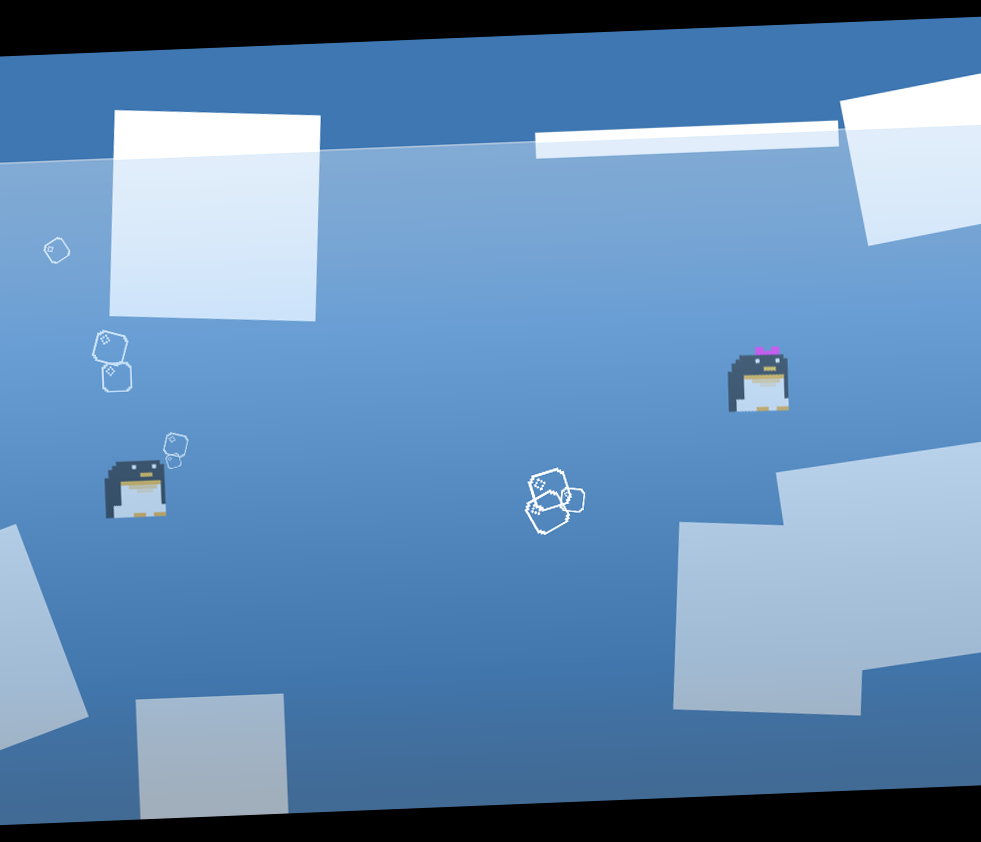
\includegraphics[width=0.45\textwidth]{img/02_mockup.png}
            }
            \caption{Concept}
            \label{fig:concepts}
        \end{figure}

\clearpage

    \subsection{Early game prototype}
        See Fig. \ref{fig:prototype_screenshots}
        \begin{figure}[h]
            % \subfloat[Early prototype]{
                % \includegraphics[width=0.45\textwidth]{img/03_prototype_screenshot.png}
            % }
            \subfloat[Early game assets]{
                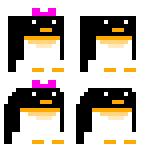
\includegraphics[width=0.45\textwidth]{img/04_penguin_assets.png}
            }
            \subfloat[Prototype using first few assets]{
                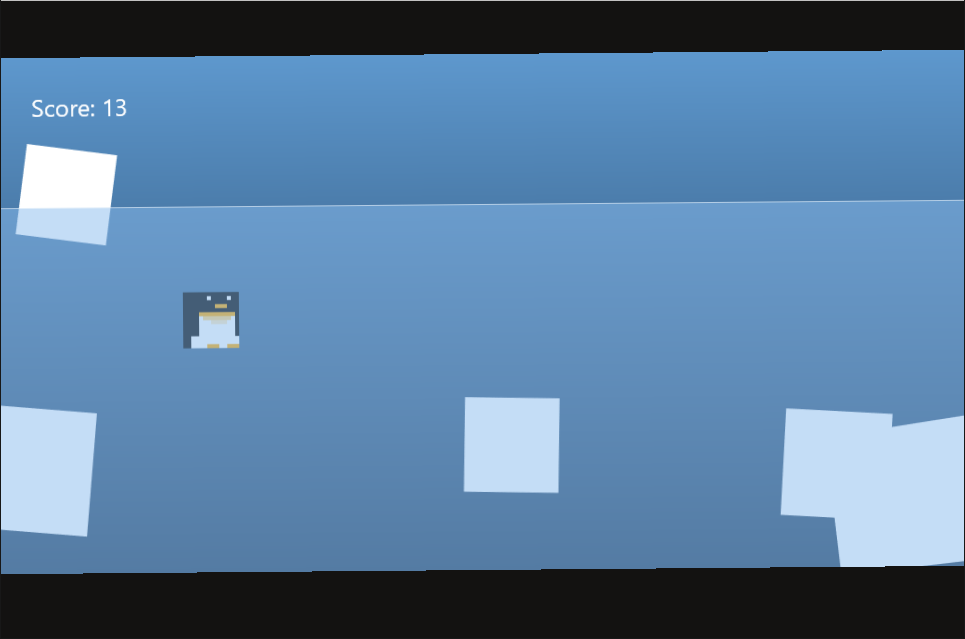
\includegraphics[width=0.45\textwidth]{img/05_prototype_screenshot.png}
            }
            \subfloat[Prototype using first few assets]{
                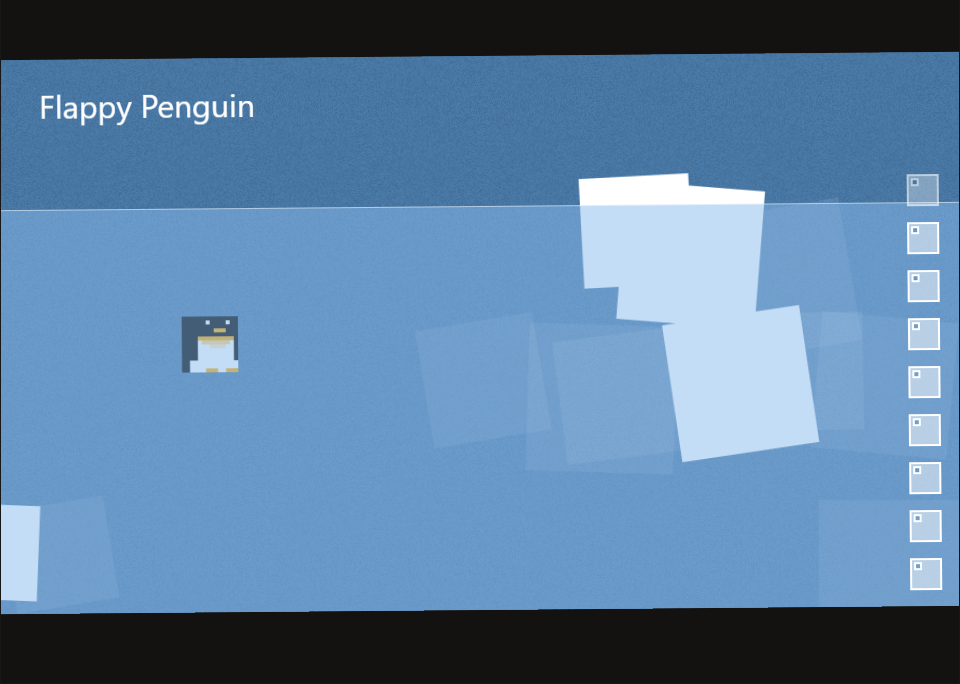
\includegraphics[width=0.45\textwidth]{img/06_prototype_screenshot.png}
            }
            \caption{Screenshots of different iterations}
            \label{fig:prototype_screenshots}
        \end{figure}

\section{Week 2 (6/27/16 - 7/3/16)}
    This weeks tasks:
    \begin{itemize}
        \item Incremental improvements of the game
        \item Breathing sensor integration
        \item Bend sensor integration
    \end{itemize}

    \subsection{Game improvements}
        By now the game includes the following components
        \begin{itemize}
            \item Basic scene layout
            \item Jumping by keyboard input
            \item Random obstacle generation
            \item Obstacle collision
            \item Breath and Breath GUI
            \item Pausing
        \end{itemize}

        Using a\em NodeJS\em server data is sent from the\em Arduino\em to the game via \em Socket.IO\em.

        With this we are now able to decrease the breath-meter when the user breathes while the penguin is beneath the water surface and increase it when it is above.

\end{document}
